
\chapter{Results} \label{chap:result}

\section{Method}

For benchmarking two metrics where measured:

\begin{itemize}
	\item Time \\
	      Time until a solution is found.
	\item Iterations \\
	      How many times the recursive algorithm was called.
\end{itemize}

For time measurments hyperfine~\cite{hyperfine:2023} is used. Each benchmark includes 3 warmup runs and is averaged. The longer the solver takes, the fewer runs are done. This is default behaviour of hyperfine. At least 10 runs made were made for each benchmark. Time is usually given in seconds. More time is worse. Iterations were measured by doing 5 runs and averaging the number of iterations used. More iterations is worse.

A benchmark is a pair of problem size with a combination of algorithmic modifications to the solver. As Oxiflex allows to enable each optimization we can create 8 optimization combinations. Note that by default the all optimizations are enabled and by passing flags to Oxiflex we disable them.

\begin{itemize}
	\item \verb|-n -r| \\
	      NaiveBacktracking
	\item \verb|-n| \\
	      NaiveBacktracking with variable ordering
	\item \verb|-f -r| \\
	      Inference with forward checking
	\item \verb|-f| \\
	      Inference with forward checking and variable ordering
	\item \verb|-a 1 -r| \\
	      Inference with AC-1
	\item \verb|-a 1| \\
	      Inference with AC-1 and variable ordering
	\item \verb|-r| \\
	      Inference with AC-3
	\item \verb|no flags| \\
	      Inference with AC-3 and variable ordering
\end{itemize}

The following Problem Domains where measured:

\begin{itemize}
	\item N-Queens
	\item Slow Convergence
\end{itemize}

All benchmark were performed on the same machine. \\

\begin{tabular}{>{\hspace{1em}}l l}
	CPU:               & Intel i7-6700K (8) @ 4.200GHz \\
	Memory:            & 6051MiB / 32021MiB            \\
	hyperfine version: & 1.16.1                        \\
	Rust version:      & 1.76.0                        \\
	Operating System:  & Pop!\_OS 22.04 LTS
\end{tabular}

\section{N-Queens}

Figure~\ref{fig:queens:time} shows the N-Queens Problem (See~\ref{sec:queens}:~\nameref{sec:queens}) with $n = 4..14$. Figure~\ref{fig:queens:iterations} shows benchmarks with the same parameters for measurements of iterations.

\begin{figure}[ht]
	\centering
	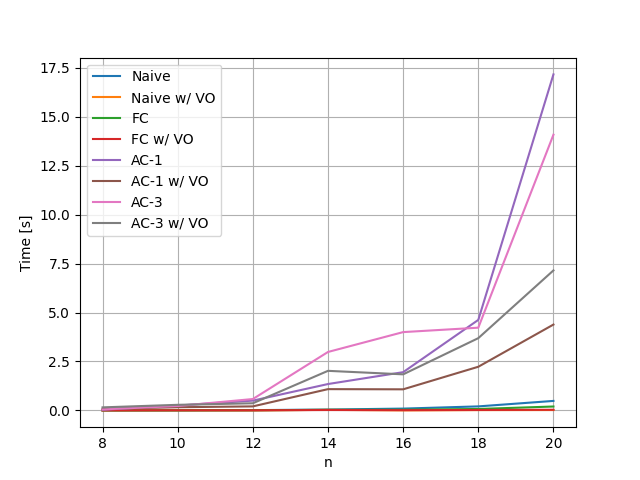
\includegraphics[width=0.8\textwidth]{./Problems/queens/plots/time.png}
	\caption{Time measurements with all possible flag combinations}
	\label{fig:queens:time}
\end{figure}

\begin{figure}[ht]
	\centering
	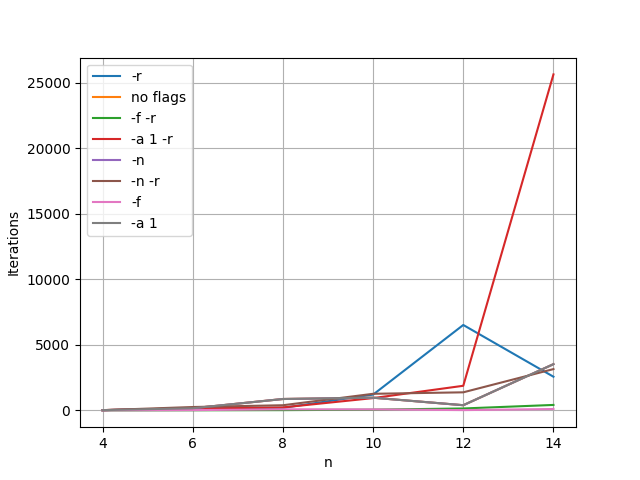
\includegraphics[width=0.8\textwidth]{./Problems/queens/plots/iterations.png}
	\caption{Iteration measurements with all possible flag combinations}
	\label{fig:queens:iterations}
\end{figure}

It appears that the time measuments in Figure~\ref{fig:queens:time} for runs that do not enforce arc consistency grow linearly. Figure~\ref{fig:queens:time_no_arc} shows benchmarks only for runs that do not enfore arc consistency using the same steps for $n$.

\begin{figure}[ht]
	\centering
	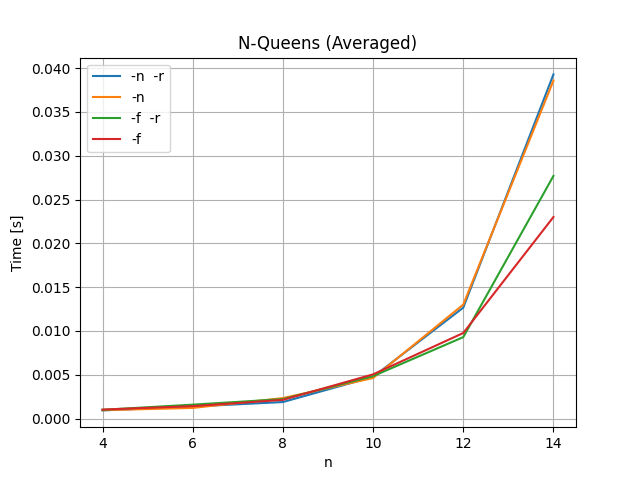
\includegraphics[width=0.8\textwidth]{./Problems/queens/plots/time_no_arc.png}
	\caption{Time measurements without arc consistency enforcing flags}
	\label{fig:queens:time_no_arc}
\end{figure}

\begin{figure}[ht]
	\centering
	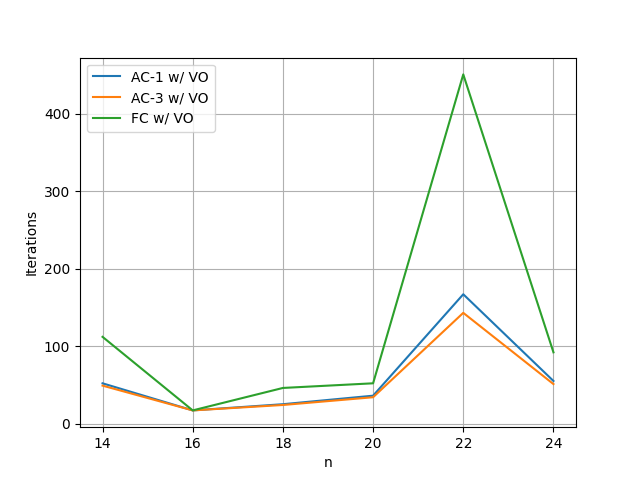
\includegraphics[width=0.8\textwidth]{./Problems/queens/plots/iterations_inference.png}
	\caption{Iterations only for inference methods}
	\label{fig:queens:iterations_inference}
\end{figure}

Table~\ref{tab:queens:time} and table~\ref{tab:queens:iterations} contains results for time and iterations. Time values are rounded to 2 decimal places.

\begin{table}[h!]
	\centering
	\begin{tabular}{|c|c|c|c|c|c|c|}
		\hline
		n           & 14              & 16              & 18              & 20                \\ \hline
		Naive       & 0.05 $\pm$ 0.08 & 0.09 $\pm$ 0.12 & 0.21 $\pm$ 0.45 & 0.49 $\pm$ 1.29   \\ \hline
		FC          & 0.03 $\pm$ 0.03 & 0.04 $\pm$ 0.04 & 0.07 $\pm$ 0.10 & 0.20 $\pm$ 0.66   \\ \hline
		AC-1        & 1.35 $\pm$ 0.73 & 1.95 $\pm$ 1.06 & 4.62 $\pm$ 3.25 & 17.17 $\pm$ 31.87 \\ \hline
		AC-3        & 2.99 $\pm$ 1.92 & 4.00 $\pm$ 2.67 & 4.23 $\pm$ 0.97 & 14.09 $\pm$ 9.93  \\ \hline
		Naive w/ VO & 0.03            & 0.00            & 0.02            & 0.02              \\ \hline
		FC w/ VO    & 0.02            & 0.01            & 0.02            & 0.03              \\ \hline
		AC1 w/ VO   & 1.09 $\pm$ 0.02 & 1.08 $\pm$ 0.03 & 2.23 $\pm$ 0.04 & 4.39 $\pm$ 0.06   \\ \hline
		AC3 w/ VO   & 2.02 $\pm$ 0.04 & 1.84 $\pm$ 0.05 & 3.69 $\pm$ 0.06 & 7.15 $\pm$ 0.05   \\ \hline
	\end{tabular}
	\caption{N-Queens Time in seconds}
	\label{tab:queens:time}
\end{table}

\begin{table}[h!]
	\centering
	\begin{tabular}{|c|c|c|c|c|c|c|}
		\hline
		n           & 14              & 16             & 18              & 20                \\ \hline
		Naive       & 3538 $\pm$ 1148 & 1749 $\pm$ 907 & 2760 $\pm$ 1145 & 21479 $\pm$ 11183 \\ \hline
		FC          & 110 $\pm$ 51    & 415 $\pm$ 76   & 79 $\pm$ 16     & 270 $\pm$ 63      \\ \hline
		AC-1        & 51 $\pm$ 9      & 396 $\pm$ 343  & 195 $\pm$ 67    & 104 $\pm$ 19      \\ \hline
		AC-3        & 103 $\pm$ 41    & 34 $\pm$ 6     & 91 $\pm$ 68     & 86 $\pm$ 30       \\ \hline
		Naive w/ VO & 3536            & 137            & 1018            & 1011              \\ \hline
		FC w/ VO    & 112             & 17             & 46              & 52                \\ \hline
		AC1 w/ VO   & 52              & 17             & 25              & 36                \\ \hline
		AC3 w/ VO   & 49              & 17             & 24              & 34                \\ \hline
	\end{tabular}
	\caption{N-Queens Iterations}
	\label{tab:queens:iterations}
\end{table}
% TODO: Notice how -n -a1 and noflags all have same

\section{Slow Convergence}

The Slow Convergence Problem is from the minizinc benchmarks repository~\cite{minizinc_slow:2018}. Benchmarks without variable ordering took way to long and are therefore omitted. Figure~\ref{fig:slow:time_small} therefore only shows benchmarks with variable ordering enabled for $n=1..10$, as higher values for $n$ took way to long to measure. Note that the benchmark repo suggests \verb|dzn| files for $n$ values from $100$ up to $1000$.

Figure~\ref{fig:slow:iterations_small} shows benchmarks with the same parameters for measurments of iterations. Note the huge spike in iterations at $n = 3$. This spike is not a measurement error. The benchmarks were run multiple times and provided the same results.

\begin{figure}[ht]
	\centering
	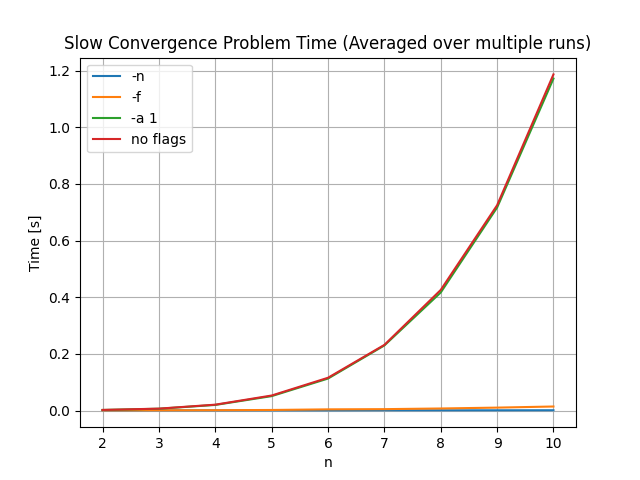
\includegraphics[width=0.8\textwidth]{./Problems/slow_convergence/plots/time_small.png}
	\caption{Time measurements only with varaible ordering combinations}
	\label{fig:slow:time_small}
\end{figure}

\begin{figure}[ht]
	\centering
	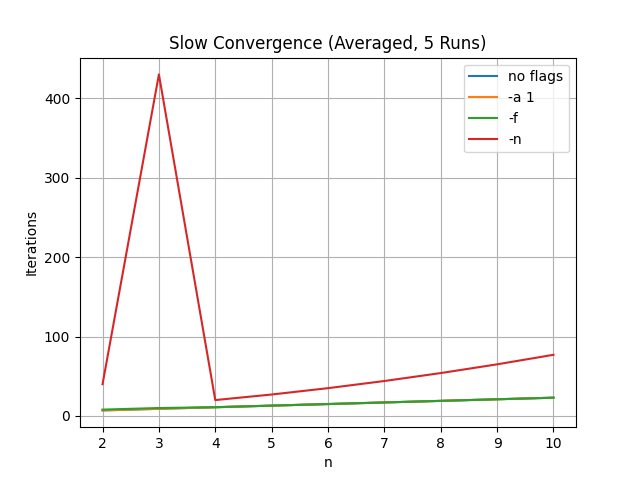
\includegraphics[width=0.8\textwidth]{./Problems/slow_convergence/plots/iterations_small.png}
	\caption{Iteration measurements only with varaible ordering combinations}
	\label{fig:slow:iterations_small}
\end{figure}

Next increasing $n$ for non arc consistency enforcing benchmarks. Figure~\ref{fig:slow:sidebyside} shows time measurements on the left and iteration measurements on the right. Note the inverse correlation between iterations and time for the two options. Altough naive backtracking (\verb|-n|) takes more iterations, it is still faster than forward checking (\verb|-f|).

\begin{figure}[ht]
	\centering
	\begin{minipage}{0.49\textwidth}
		\centering
		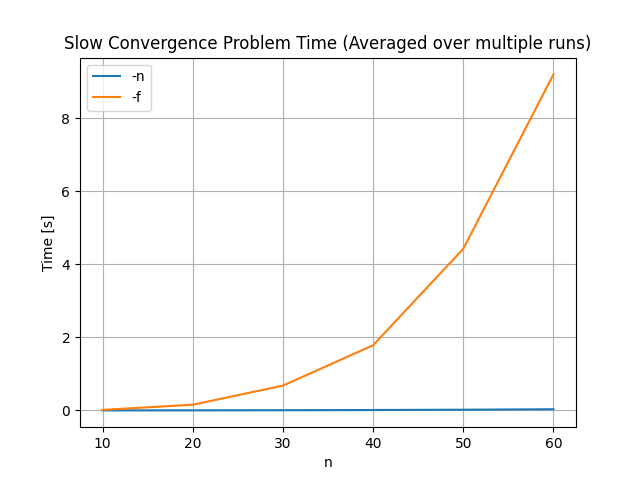
\includegraphics[width=\textwidth]{./Problems/slow_convergence/plots/time.png}
	\end{minipage}
	\hfill
	\begin{minipage}{0.49\textwidth}
		\centering
		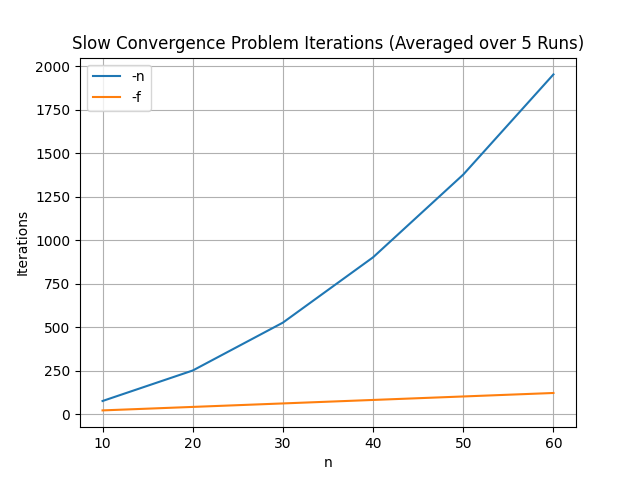
\includegraphics[width=\textwidth]{./Problems/slow_convergence/plots/iterations.png}
	\end{minipage}
	\caption{Comparison for higher $n = 10..60$. Left: time, right: iterations.}
	\label{fig:slow:sidebyside}
\end{figure}

~\cref{tab:slow:time} and ~\cref{tab:slow:iterations} contain results for time and iterations for the $n = 10..60$ range. Time values are rounded to 2 decimal places.

\begin{table}[h!]
	\centering
	\begin{tabular}{c c}
		\begin{minipage}{.5\textwidth}
			\centering
			\begin{tabular}{| c | c | c |}
				\hline
				n  & Naive w/ VO & FC w/ VO        \\ \hline
				10 & 0.00        & 0.01            \\ \hline
				20 & 0.00        & 0.13            \\ \hline
				30 & 0.01        & 0.54 $\pm$ 0.01 \\ \hline
				40 & 0.01        & 1.58 $\pm$ 0.08 \\ \hline
				50 & 0.02        & 5.29 $\pm$ 0.14 \\ \hline
				60 & 0.04        & 21.94 $\pm$ 0.5 \\ \hline
			\end{tabular}
			\caption{Slow Convergence Time}
			\label{tab:slow:time}
		\end{minipage} &
		\begin{minipage}{.5\textwidth}
			\centering
			\begin{tabular}{| c | c | c |}
				\hline
				n  & Naive w/ VO & FC w/ VO \\ \hline
				10 & 77          & 23       \\ \hline
				20 & 252         & 43       \\ \hline
				30 & 527         & 63       \\ \hline
				40 & 902         & 83       \\ \hline
				50 & 1377        & 103      \\ \hline
				60 & 1952        & 123      \\ \hline
			\end{tabular}
			\caption{Slow Convergence Iterations}
			\label{tab:slow:iterations}
		\end{minipage}
	\end{tabular}
\end{table}

For comparison figure~\ref{fig:slow:gecode} shows Oxiflex compared to Gecode. Gecode is a constraint satisfaction problem solver compatible with MiniZinc with state-of-the art performance~\cite{gecode}. Note the steep increase in $n = 100..600$.

\begin{figure}[ht]
	\centering
	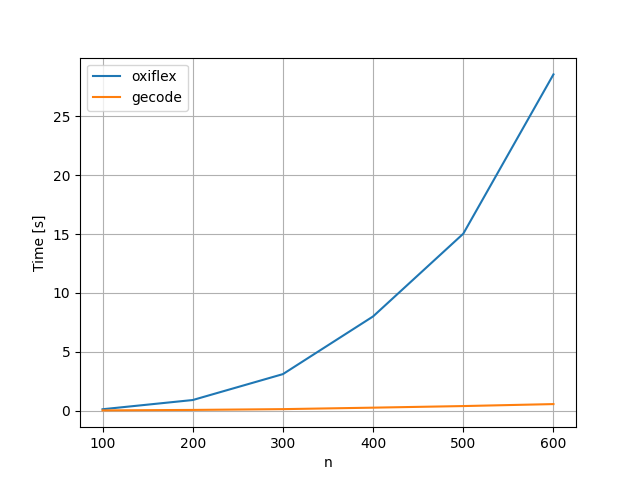
\includegraphics[width=0.8\textwidth]{./Problems/slow_convergence/plots/gecode.png}
	\caption{Oxiflex vs gecode}
	\label{fig:slow:gecode}
\end{figure}
